\documentclass{ntuthesis}

% <commands>



\newcommand{\ind}{\hphantom{aaaa}}

\newcommand{\todo}[1]{\noindent\textcolor{ForestGreen}{TODO:} \textcolor{MidnightBlue}{#1}}
\newcommand{\sketchnote}[1]{\noindent\textcolor{MidnightBlue}{#1}}
\newenvironment{sketch}{\par\color{blue}}{\par}

\newcommand{\half}{{\scriptstyle \frac{1}{2}}}
\newcommand{\paral}{{\!/\mkern-5mu/\!}}
\newcommand{\trihat}[1]{{\stackrel{\scriptscriptstyle\Delta}{#1}}}
\newcommand{\diff}[1]{{\Delta{#1}}}
\newcommand{\smallminus}{\scalebox{0.5}[1.0]{\( - \)}}
\newcommand{\invhB}{\B^{\scalebox{0.5}[1.0]{\( - \)}\frac{1}{2}}}

\newcommand{\mj}{\mathbf{j}}
\newcommand{\ma}{\mathbf{a}}
\newcommand{\p}{\mathbf{p}}
\newcommand{\q}{\mathbf{q}}
\newcommand{\qd}{{\dot{\q}}}
\newcommand{\qdd}{{\ddot{\q}}}
\newcommand{\uu}{\mathbf{u}}
\newcommand{\ud}{{\dot{\uu}}}
\newcommand{\udd}{{\ddot{\uu}}}
\newcommand{\vv}{\mathbf{v}}
\newcommand{\vd}{{\dot{\vv}}}
\newcommand{\vdd}{{\ddot{\vv}}}
\newcommand{\x}{\mathbf{x}}
\newcommand{\xd}{{\dot{\x}}}
\newcommand{\xdd}{{\ddot{\x}}}
\newcommand{\y}{\mathbf{y}}
\newcommand{\yd}{{\dot{\y}}}
\newcommand{\ydd}{{\ddot{\y}}}
\newcommand{\z}{\mathbf{z}}
\newcommand{\zd}{{\dot{\z}}}
\newcommand{\zdd}{{\ddot{\z}}}
\newcommand{\mb}{\mathbf{b}}
\newcommand{\mr}{\mathbf{r}}
\newcommand{\s}{\mathbf{s}}
\newcommand{\sd}{{\dot{\s}}}
\newcommand{\sdd}{{\ddot{\s}}}
\newcommand{\oo}{\mathbf{o}}
\newcommand{\f}{\mathbf{f}}
\newcommand{\h}{\mathbf{h}}
\newcommand{\g}{\mathbf{g}}
\newcommand{\mc}{\mathbf{c}}
\newcommand{\ml}{\mathbf{l}}
\newcommand{\mt}{\mathbf{t}}
\newcommand{\mlambda}{\mathbf{\lambda}}
\newcommand{\torq}{\mathbf{\tau}}
\newcommand{\zero}{\mathbf{0}}
\newcommand{\one}{\mathbf{1}}
\newcommand{\Real}{\mathbb{R}}
\newcommand{\J}{\mathbf{J}}
\newcommand{\Jd}{{\dot{\J}}}
\newcommand{\Jp}{\J_{\phi}}
\newcommand{\Jdp}{\Jd_{\phi}}
\newcommand{\A}{\mathbf{A}}
\newcommand{\B}{\mathbf{B}}
\newcommand{\C}{\mathbf{C}}
\newcommand{\D}{\mathbf{D}}
\newcommand{\F}{\mathbf{F}}
\newcommand{\G}{\mathbf{G}}
\newcommand{\mH}{\mathbf{H}}
\newcommand{\I}{\mathbf{I}}
\newcommand{\mL}{\mathbf{L}}
\newcommand{\M}{\mathbf{M}}
\newcommand{\U}{\mathbf{U}}
\newcommand{\mR}{\mathbf{R}}
\newcommand{\mS}{\mathbf{S}}
\newcommand{\mT}{\mathbf{T}}
\newcommand{\V}{\mathbf{V}}
\newcommand{\W}{\mathbf{W}}
\newcommand{\bfzero}{\mathbf{0}}
\newcommand{\inner}[2]{\langle#1,#2\rangle}
\newcommand{\wt}[1]{{\widetilde{#1}}}
\newcommand{\wh}[1]{{\widehat{#1}}}

\newcommand{\T}{\top}

\newcommand{\calQ}{{\cal Q}}
\newcommand{\calC}{{\cal C}}
\newcommand{\calR}{{\cal R}}
\newcommand{\calU}{{\cal U}}
\newcommand{\calX}{{\cal X}}
\newcommand{\calZ}{{\cal Z}}
\newcommand{\calL}{{\cal L}}
\newcommand{\calH}{{\cal H}}



% last update: 2018-06-10
% created by Ching-An Cheng

% PACKAGES
% math
\usepackage{amsmath}
\usepackage{amsfonts}
\usepackage{amssymb}
\usepackage{amsthm}
\usepackage{bm}
\usepackage{bbm}
\usepackage{mathtools}
\usepackage{enumitem}
\usepackage{thmtools,thm-restate}
% algorithms
\usepackage{algorithm}
\usepackage{algorithmic}
% ref
%\usepackage{natbib}
% misc
\usepackage{color}
\usepackage{graphicx}
\usepackage{comment}
%\usepackage[latin1]{inputenc} % for German


% EDITS
%\newcommand{\todo}[1]{{\leavevmode\color{red}TODO: #1}}
\newcommand{\rev}[1]{{\leavevmode\color{blue}#1}}

% SHORTCUTS
% theorem setting
\renewcommand\qedsymbol{$\blacksquare$}

%\theoremstyle{plain}
%\newtheorem{lemma}{Lemma}[section]
%\newtheorem{theorem}{Theorem}[section]
%\newtheorem{proposition}{Proposition}[section]
%\newtheorem{corollary}{Corollary}[section]

%\theoremstyle{definition}
%newtheorem{definition}{Definition}[section]
%\newtheorem{example}{Example}[section]

%\theoremstyle{remark}
%\newtheorem{remark}{Remark}[section]
\newtheorem{assumption}{Assumption}[section]

\newenvironment{proofsketch}{\textit{Proof sketch:}}{\qed \par}


% fonts
\def\AA{\mathcal{A}}\def\BB{\mathcal{B}}\def\CC{\mathcal{C}}
\def\DD{\mathcal{D}}\def\EE{\mathcal{E}}\def\FF{\mathcal{F}}
\def\GG{\mathcal{G}}\def\HH{\mathcal{H}}\def\II{\mathcal{I}}
\def\JJ{\mathcal{J}}\def\KK{\mathcal{K}}\def\LL{\mathcal{L}}
\def\MM{\mathcal{M}}\def\NN{\mathcal{N}}\def\OO{\mathcal{O}}
\def\PP{\mathcal{P}}\def\QQ{\mathcal{Q}}\def\RR{\mathcal{R}}
\def\SS{\mathcal{S}}\def\TT{\mathcal{T}}\def\UU{\mathcal{U}}
\def\VV{\mathcal{V}}\def\WW{\mathcal{W}}\def\XX{\mathcal{X}}
\def\YY{\mathcal{Y}}\def\ZZ{\mathcal{Z}}

\def\Ab{\mathbf{A}}\def\Bb{\mathbf{B}}\def\Cb{\mathbf{C}}
\def\Db{\mathbf{D}}\def\Eb{\mathbf{E}}\def\Fb{\mathbf{F}}
\def\Gb{\mathbf{G}}\def\Hb{\mathbf{H}}\def\Ib{\mathbf{I}}
\def\Jb{\mathbf{J}}\def\Kb{\mathbf{K}}\def\Lb{\mathbf{L}}
\def\Mb{\mathbf{M}}\def\Nb{\mathbf{N}}\def\Ob{\mathbf{O}}
\def\Pb{\mathbf{P}}\def\Qb{\mathbf{Q}}\def\Rb{\mathbf{R}}
\def\Sb{\mathbf{S}}\def\Tb{\mathbf{T}}\def\Ub{\mathbf{U}}
\def\Vb{\mathbf{V}}\def\Wb{\mathbf{W}}\def\Xb{\mathbf{X}}
\def\Yb{\mathbf{Y}}\def\Zb{\mathbf{Z}}\def\0b{\mathbf{0}}

\def\ab{\mathbf{a}}\def\bb{\mathbf{b}}\def\cb{\mathbf{c}}
\def\db{\mathbf{d}}\def\eb{\mathbf{e}}\def\fb{\mathbf{f}}
\def\gb{\mathbf{g}}\def\hb{\mathbf{h}}\def\ib{\mathbf{i}}
\def\jb{\mathbf{j}}\def\kb{\mathbf{k}}\def\lb{\mathbf{l}}
\def\mbb{\mathbf{m}}
\def\nb{\mathbf{n}}\def\ob{\mathbf{o}}
\def\pb{\mathbf{p}}\def\qb{\mathbf{q}}\def\rb{\mathbf{r}}
\def\sbb{\mathbf{s}} % some conflicts with url
\def\tb{\mathbf{t}}\def\ub{\mathbf{u}}
\def\vb{\mathbf{v}}\def\wb{\mathbf{w}}\def\xb{\mathbf{x}}
\def\yb{\mathbf{y}}\def\zb{\mathbf{z}}

\def\Abb{\mathbb{A}}\def\Bbb{\mathbb{B}}\def\Cbb{\mathbb{C}}
\def\Dbb{\mathbb{D}}\def\Ebb{\mathbb{E}}\def\Fbb{\mathbb{F}}
\def\Gbb{\mathbb{G}}\def\Hbb{\mathbb{H}}\def\Ibb{\mathbb{I}}
\def\Jbb{\mathbb{J}}\def\Kbb{\mathbb{K}}\def\Lbb{\mathbb{L}}
\def\Mbb{\mathbb{M}}\def\Nbb{\mathbb{N}}\def\Obb{\mathbb{O}}
\def\Pbb{\mathbb{P}}\def\Qbb{\mathbb{Q}}\def\Rbb{\mathbb{R}}
\def\Sbb{\mathbb{S}}\def\Tbb{\mathbb{T}}\def\Ubb{\mathbb{U}}
\def\Vbb{\mathbb{V}}\def\Wbb{\mathbb{W}}\def\Xbb{\mathbb{X}}
\def\Ybb{\mathbb{Y}}\def\Zbb{\mathbb{Z}}

\def\Af{\mathfrak{A}}\def\Bf{\mathfrak{B}}\def\Cf{\mathfrak{C}}
\def\Df{\mathfrak{D}}\def\Ef{\mathfrak{E}}\def\Ff{\mathfrak{F}}
\def\Gf{\mathfrak{G}}\def\Hf{\mathfrak{H}}\def\If{\mathfrak{I}}
\def\Jf{\mathfrak{J}}\def\Kf{\mathfrak{K}}\def\Lf{\mathfrak{L}}
\def\Mf{\mathfrak{M}}\def\Nf{\mathfrak{N}}\def\Of{\mathfrak{O}}
\def\Pf{\mathfrak{P}}\def\Qf{\mathfrak{Q}}\def\Rf{\mathfrak{R}}
\def\Sf{\mathfrak{S}}\def\Tf{\mathfrak{T}}\def\Uf{\mathfrak{U}}
\def\Vf{\mathfrak{V}}\def\Wf{\mathfrak{W}}\def\Xf{\mathfrak{X}}
\def\Yf{\mathfrak{Y}}\def\Zf{\mathfrak{Z}}

% math 
\def\R{\Rbb}
\def\Q{\Qbb}\def\Z{\Zbb}\def\N{\Nbb}
%\def\C{\Cbb}
%\def\one{{\mathbbm1}}
\def\GP{\GG\PP}
\def\K{\mathcal{K}}
\def\der{\mathrm{d}}
\def\zinf{[0, \infty) }
\def\afsystem{\dot{x}  =f(x) + g(x)u}
\def\const{\mathrm{const.}}
\def\diag{\mathrm{diag}}
\def\bdiag{\mathrm{blkdiag}}
\def\mvec{\mathrm{vec}}
\def\t{\top}
\def\*{\star}


\newcommand{\norm}[1]{ \| #1 \|  }
\newcommand{\abs}[1]{ \left| #1 \right|  }
\newcommand{\tr}[1]{ \mathrm{tr}\left( #1\right)}
\newcommand{\lr}[2]{ \left\langle #1, #2 \right\rangle}
\DeclareMathOperator*{\argmin}{arg\,min}
\DeclareMathOperator*{\argmax}{arg\,max}


% online learning
\def\regret{\textrm{Regret}}

% statistics
\newcommand{\KL}[2]{D_{KL}(#1, #2)} %\newcommand{\KL}[2]{KL[#1 || #2  ]}
\newcommand{\TV}[2]{D_{TV}(#1, #2)}
\newcommand{\HE}[2]{D_{H}(#1, #2)}
\newcommand{\WA}[2]{D_{W}(#1, #2)}
\newcommand{\FD}[2]{D_{f}(#1, #2)}
\newcommand{\E}{\Ebb}
\newcommand{\Var}{\mathrm{Var}}
\newcommand{\Cov}{\mathrm{Cov}}


%% Below is the code for optionally collecting all the proofs at the end
%% source: https://tex.stackexchange.com/questions/33229/how-to-place-all-proofs-automatically-in-appendix
%\usepackage{etex,etoolbox}
%%\usepackage{amsthm,amssymb}
%%\usepackage{thmtools}
%\usepackage{environ}
%
%\makeatletter
%\providecommand{\@fourthoffour}[4]{#4}
%% We define an addition for the theorem-like environments; when
%% \newtheorem{thm}{Theorem} is declared, the macro \thm expands
%% to {...}{...}{...}{Theorem} and with \@fourthoffour we access
%% to it; then we make available \@currentlabel (the theorem number)
%% also outside the environment.  
%\newcommand\fixstatement[2][\proofname\space of]{%
%	\ifcsname thmt@original@#2\endcsname
%	% the theorem has been declared with \declaretheorem
%	\AtEndEnvironment{#2}{%
%		\xdef\pat@label{\expandafter\expandafter\expandafter
%			\@fourthoffour\csname thmt@original@#2\endcsname\space\@currentlabel}%
%		\xdef\pat@proofof{\@nameuse{pat@proofof@#2}}%
%	}%
%	\else
%	% the theorem has been declared with \newtheorem
%	\AtEndEnvironment{#2}{%
%		\xdef\pat@label{\expandafter\expandafter\expandafter
%			\@fourthoffour\csname #1\endcsname\space\@currentlabel}%
%		\xdef\pat@proofof{\@nameuse{pat@proofof@#2}}%
%	}%
%	\fi
%	\@namedef{pat@proofof@#2}{#1}%
%}
%
%% We allocate a block of 1000 token registers; in this way \prooftoks
%% is 1000 and we can access the following registers of the block by
%% \prooftoks+n (0<n<1000); we'll use a dedicated counter for it
%% that is stepped at every proof
%\globtoksblk\prooftoks{1000}
%\newcounter{proofcount}
%
%% We gather the contents of the proof as argument to \proofatend
%% and then we store
%% "\begin{proof}[Proof of <theoremname> <theoremnumber>]#1\end{proof}"
%% in the next token register of the allocated block
%\NewEnviron{proofatend}{%
%	\edef\next{%
%		\noexpand\begin{proof}[\pat@proofof\space\pat@label]%
%			\unexpanded\expandafter{\BODY}}%
%		\global\toks\numexpr\prooftoks+\value{proofcount}\relax=\expandafter{\next\end{proof}}
%	\stepcounter{proofcount}}
%
%% \printproofs simply loops over the used token registers of the
%% block, freeing their contents
%\def\printproofs{%
%	\count@=\z@
%	\loop
%	\the\toks\numexpr\prooftoks+\count@\relax
%	\ifnum\count@<\value{proofcount}%
%	\advance\count@\@ne
%	\repeat}
%\makeatother
%
%%% Here starts the example, with two theorem declarations
%%\declaretheorem[style=plain,name=Theorem,qed=$\square$,numberwithin=section]{thm}
%%%\declaretheorem[style=plain,name=Lemma,qed=$\square$,numberlike=thm]{lem}
%%%\newtheorem{thm}{Theorem}
%%\newtheorem{lem}[thm]{Lemma}
%%\fixstatement{thm}
%%\fixstatement[Demonstration of]{lem}
%
%\fixstatement{lemma}
%\fixstatement{theorem}
%\fixstatement{proposition}
%\fixstatement{corollary}

\usepackage{times}
\usepackage{verbatim}
\usepackage{color}
\usepackage{url}
\usepackage{graphicx}
\usepackage{array}
\usepackage{wallpaper}
\usepackage{hyperref}
\usepackage[printwatermark]{xwatermark}
\usepackage{graphicx}
\usepackage{tikz}

% Using the tex-text mapping for ligatures etc.
\defaultfontfeatures{Mapping=tex-text}

% Set the default fonts
\setmainfont{Times New Roman}
\setCJKmainfont[AutoFakeBold=true,AutoFakeSlant=true]{BiauKai}
%\setCJKmainfont[BoldFont={粗楷體},ItalicFont={斜楷體}]{標楷體}

\ifdefined\firstpage

  \ifdefined\withwatermark
    \newsavebox\mybox
    \savebox\mybox{\tikz[opacity=0.5]\node{\includegraphics{watermark.pdf}};}
    \newwatermark*[allpages,xpos=6.1725cm,ypos=10.5225cm,scale=0.5]{\usebox\mybox}
  \fi

  % digital object identifier
  \ifdefined\withdoi
    \insertdoi
  \fi
\fi

\makeatletter
\AtBeginDocument{
  \hypersetup{
    pdftitle={\@titleen},
    pdfauthor={\@authoren},
    pdfsubject={\@typeen{} \@classen},
    pdfkeywords={\@keywordsen}
  }
}
\makeatother

% Your information goes here
% author: Tz-Huan Huang [http://www.csie.ntu.edu.tw/~tzhuan]

% ----------------------------------------------------------------------------
% "THE CHOCOLATE-WARE LICENSE":
% Tz-Huan Huang wrote this file. As long as you retain this notice you
% can do whatever you want with this stuff. If we meet some day, and you think
% this stuff is worth it, you can buy me a chocolate in return Tz-Huan Huang
% ----------------------------------------------------------------------------

% Syntax: \var{English}{Chinese}
\university{National Taiwan University}{國立臺灣大學}
\college{College of Engineering}{}
\institute{Department of Mechanical Engineering}{机械工程學系}
\title{Robot Multi-task Control Based on Riemannian Motion Policies and Qual Quaternion}{基於黎曼運動決策和雙四元數的機器人多任務控制}
\author{Chen-Han Lin}{林晨涵}
\studentid{R07522843}
\advisor{Han-Pang Huang, Ph.D.}{黃漢邦 博士}
\defenseyear{2020}{109}
\defensemonth{June}{6}
\defenseday{28}
\doi{doi:10.6342/NTU2017XXXXX}
\keywords{keyword}{關鍵字}


\begin{document}

\frontmatter

\makecover

\ifdefined\excludefirstpage

  \ifdefined\withwatermark
    \newsavebox\mybox
    \savebox\mybox{\tikz[opacity=0.5]\node{\includegraphics{watermark.pdf}};}
    \newwatermark*[allpages,xpos=6.1725cm,ypos=10.5225cm,scale=0.5]{\usebox\mybox}
  \fi

  % digital object identifier
  \ifdefined\withdoi
    \insertdoi
  \fi
\fi

\makecertification



\newif\ifLONG
\LONGfalse

\begin{acknowledgementszh}
感謝\ldots
\end{acknowledgementszh}

\begin{acknowledgementsen}
I'm glad to thank\ldots 
\end{acknowledgementsen}

%\begin{abstractzh}
%本論文提出了一影像中使用者感興趣區域 (region of interest)
%偵測之資料集 (benchmark)。
%使用者感興趣區域偵測在許多應用中極為有用,
%過去雖然有許多使用者感興趣區域之自動偵測演算法被提出,
%然而由於缺乏公開資料集,
%這些方法往往只測試了各自的小量資料而難以互相比較。
%從其它領域可以發現,
%基於公開資料集的可重製實驗與該領域突飛猛進密切相關,
%因此本論文填補了此領域之不足,
%我們提出名為「Photoshoot」的遊戲來蒐集人們對於感興趣區域的標記,
%並以這些標記來建立資料集。
%透過這個遊戲,我們已蒐集大量使用者對於感興趣區域的標記,
%並結合這些資料成為使用者感興趣區域模型。
%我們利用這些模型來量化評估五個使用者感興趣區域偵測演算法,
%此資料集也可更進一步作為基於學習理論演算法的測試資料,
%因此使基於學習理論的偵測演算法成為可能。

\bigbreak
\noindent \textbf{關鍵字:}{\, \makeatletter \@keywordszh \makeatother}
\end{abstractzh}

\begin{abstracten}
%This thesis presents a benchmark for region of interest (ROI)
%detection. ROI detection has many useful applications and many
%algorithms have been proposed to automatically detect ROIs.
%Unfortunately, due to the lack of benchmarks, these methods were
%often tested on small data sets that are not available to others,
%making fair comparisons of these methods difficult. Examples from
%many fields have shown that repeatable experiments using published
%benchmarks are crucial to the fast advancement of the fields. To
%fill the gap, this thesis presents our design for a collaborative
%game, called Photoshoot, to collect human ROI annotations for
%constructing an ROI benchmark. With this game, we have gathered a
%large number of annotations and fused them into aggregated ROI
%models. We use these models to evaluate five ROI detection
%algorithms quantitatively. Furthermore, by using the benchmark as
%training data, learning-based ROI detection algorithms become
%viable.

\bigbreak
\noindent \textbf{Keywords:}{\, \makeatletter \@keywordsen \makeatother}
\end{abstracten}

\begin{comment}
\category{I2.10}{Computing Methodologies}{Artificial Intelligence --
Vision and Scene Understanding} \category{H5.3}{Information
Systems}{Information Interfaces and Presentation (HCI) -- Web-based
Interaction.}

\terms{Design, Human factors, Performance.}

\keywords{Region of interest, Visual attention model, Web-based
games, Benchmarks.}
\end{comment}


\tableofcontents
\listoffigures
\listoftables

\mainmatter

% Your thesis goes here
\chapter{Introduction to Multi-task Robot Control and Planning}
Unlike an industrial robot which usually execute specific tasks in a static environment, service robots face a much more complex and dynamic situation. These uncertainties and complexity required service robots to deal with multiple tasks simultaneously.
\begin{figure}
\centering
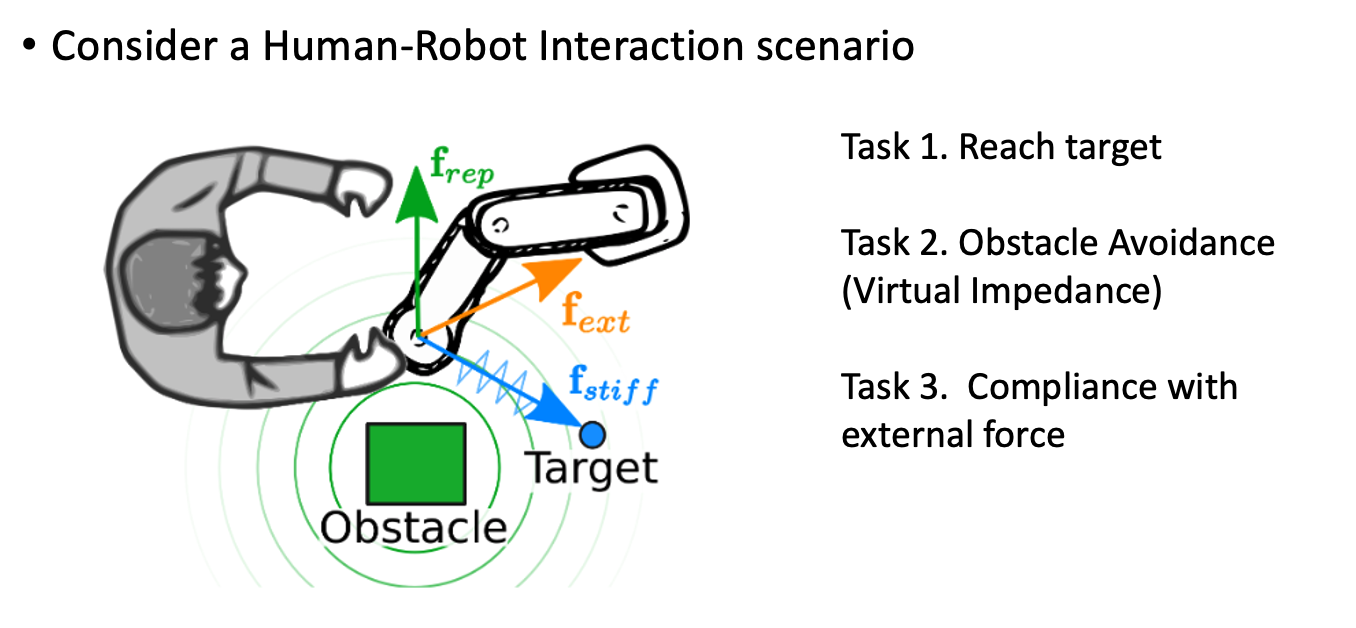
\includegraphics[width=0.55\textwidth]{images/motivation_scenario.png}
\caption{A Human-Robot interaction scenario}
\label{fig:Human-Robot interaction scenario}
\end{figure}

As Figure ~\ref{fig:Human-Robot interaction scenario} shows, a robot in this HRI scenario may have three tasks. Firstly, the robot needs to reach the target pose. Secondly, no collision is allowed to happened during the entire process (\textit{Collision Avoidance}). Lastly, to meet the safety consideration, the robot should compliance with external force imposed by humans (\textit{Compliance Control}).
 
As we can imagine, It is impossible for a robot to complete these three tasks perfectly in the same time. Either in the task space or in the configuration space, the limited variables with greater number of constraints usually return no solution. 

%ToDo citations here
A naive idea is to sum up the dynamics behavior ~\cite{Santis:2007:ASME}, but this simple idea may lead to an unstable problem, the equilibrium point is undetermined in most  cases. For example, the final pose of the robot may actually collide with obstacles.
One of the common approaches to this multi-tasks problem is null-space projection. In two tasks situation, this method isolate the first task from the second one. By treating each task in a different priority, the method project the second priority task  into the null-space of Jacobian related to the first one. 
For example, when both goal reaching and collision avoidance is considered, the \textit{task-first} type concept will place the  original robot control task in a higher priority, 
while use only the null space of Jacobian to prevent the robot from collisions. There are several problems behind this idea, it needs the robot to be highly redundant with 
respect to the task. But we can hardly find whether the null space related to original task is large enough to avoid obstacles. 
On the contrary, the \textit{avoidance-first} type approach let the original control scheme only operates in the null space of Jacobian related to collision avoidance. 
To meet safety demand in multi-priority problem, collision avoidance behavior should be set to the top priority, hence it is usually more considerable than the previous one. 
When it comes to cases where more than two tasks to be dealt with, many null-space projection based architectures were proposed to systematically handle with these tasks.
%ToDo nullspace projection method formulae
\begin{equation}
\qdd = {\Jb}^{\dagger} (\xdd - \Jd\qd)+ \mathbf{N} \qdd_0 
\end{equation}
let $\tilde{\xdd} = \xdd - \Jd\qd$
Where $\mathbf{N} = (\Ib - {\Jb}^{\dagger} \Jb)$

Many other articles  addressed  this by applying optimization based approaches. Among them, Quatratic Programming (QP) is a common choice which formulize a quaduatic math optimization 
problem by a quaduatic cost function subjected to serveral linear constraints. In the context, we may want to treat the original task as the main task, so it should be 
expressed in the cost function 
\begin{equation}
f(\qdd) = \| \Jb\qdd  - \xdd + \Jd\qd\|^2
\end{equation}
and find the $\qd = argmin_\qdd'\|\Jb\qdd' - \xdd + \Jd\qd  \|^2$ as the optimal  in no constraint cases. 


\chapter{RMP and RMPtree Concept}
\label{c:intro}

%Attention plays an important role in human vision. For example, when
%we look at an image, our eye movements comprise a succession of {\em
%fixations} (repetitive positioning of eyes to parts of the image)
%and {\em saccades} (rapid eye jump). Those parts of the image that
%cause eye fixations and capture primary attention are called {\em
%regions of interest} (ROIs). Studies in visual attention and eye
%movement have shown that humans gene	rally only attend to a few ROIs.
%Detecting these visually attentive regions in images is challenging
%but useful in many multimedia applications, such as automatic
%thumbnail cropping, object recognition, content-based image
%retrieval, adaptive image compression and automatic browsing in
%small-screen devices.
%
%Many algorithms have been proposed for automatic ROI detection in
%images. Unfortunately, these methods were often evaluated only on
%specific and small data sets that are not publicly available. The
%lack of published {\em benchmarks} makes experiments non-repeatable
%and quantitative evaluation difficult. However, as recommended by
%the latest ACM SIGMM retreat, repeatable experiments using published
benchmarks are important for advancing the multimedia research
field~\cite{Rowe:2005:ASR}.

\section{Preliminary}

Let $\mathbf{q}(t) \in \mathcal{C}  \subset \mathbb{R}^{n}$  denotes the generalized coordinates of the system in the configuration space $ \mathcal{C}$. Typically $\mathbf{q}$ contains the joint angles. 
Let us assume that there is a task space $\mathcal{T}$ which is a set of non-linear subtask spaces, denotes $\{\mathcal{T}_i\}$, and let $\mathbf{x}_i(t) \in \ \mathcal{T}_{i} \, \subseteq \, \mathbb{R}^{m_i}$ denotes the $m_i$-dimensional task variable in the $i^{th}$  subtask space at time $t$.
And the differentiable task map $\phi_i : \mathcal{C} \rightarrow \mathcal{T}_i $ relates the configuration space and $i^{th}$ subtask space. For example, if $\mathbf{x}_{i}$ is the position and orientation of the end-effector, then $\phi_{i}$ represents the forward kinematics of the robot.

If we denotes the Jacobian of a task map $\phi$ as
$\mathbf{J}_{\phi} = \frac{\partial \phi}{\partial  \mathbf{q}} \in \mathbb{R}^{k \times d},$ 
then the task space velocity and acceleration are given by
\begin{equation}
\dot{\mathbf{x}} = \mathbf{J}_{\phi}\dot{\mathbf{q}}
\end{equation}

\begin{equation}
\ddot{\mathbf{x}} = \mathbf{J}_{\phi}\ddot{\mathbf{q}} + \dot{\mathbf{J}}_{\phi}\dot{\mathbf{q}}
\end{equation}

\section{Riemannian Motion Policies}

An Riemannian Motion Policy (RMP) in its \textit{canonical form} is a motion policy denoted by the tuple $(\mathbf{a}, \mathbf{M})^{\mathcal{M}}$, is a motion policy $\mathbf{a}$ in a manifold $\mathcal{M}$ augmented by a Riemannian metric $\mathbf{M}$.

\subsection{Motion Policy}
A \textit{motion policy} $\mathbf{a} : \mathbf{x}, \dot{\mathbf{x}} \longmapsto \ddot{\mathbf{x}} $ can be seen as a second-order dynamical system in a task space $\mathcal{X}$, which maps position and velocity to acceleration. If task map $\phi$ is the identity map, we can write $\mathbf{a}:\mathbf{q},\dot{\mathbf{q}} \longmapsto \ddot{\mathbf{q}}$ without loss of generality.  

\begin{itemize}

\item A motion policy $\mathbf{a}$ is given by the user to specify a desire motion of the robot. For example, \textit{Virtual Impedance}, \textit{Collision Avoidance}, \textit{Redundancy Resolution} etc.


\item Each motion policy $\mathbf{a}(\mathbf{x}, \dot{\mathbf{x}}) $ is in a specified task space $\mathcal{X}$, For example,  \textit{Target Position dynamics} (e.g. Impedance Control) should be imposed in one of the task space, while \textit{Redundancy Resolution}  typically  takes place in the configuration space.

%% ToDo 
%% Motion Policies V.S. Trajectory Planning 

\end{itemize}
Comparing to open-loop trajectory planning methods, motion policy could be considered as a closed-loop motion behavior that depends on current state of the robot. It is obviously to say that closed-loop motion policies are more robust than trajectory planning when the robot is performing tasks in a complicated scenario.
\subsection{Riemannian Metric}

In Riemannian Geometry, the Riemannian Metric $\mathbf{M}(\mathbf{x}, \dot{\mathbf{x}})$ is a symmetric positive semidefinite matrix defined on the tangent space that measures the inner product between two tangent vectors $\mathbf{u}$ and $\mathbf{v}$ as $\langle \mathbf{u}, \mathbf{v} \rangle_{\mathbf{M}} = \mathbf{u}^T \mathbf{M} \mathbf{v}$. Thus, $\| \mathbf{u}\|^{2}_{\mathbf{M}} = \mathbf{u}^T \mathbf{M} \mathbf{u}$. \\[3mm]
For example, for a given Riemannian metric $\mathbf{M}$, we have $\dot{\mathbf{x}}^{T} \mathbf{M} \dot{\mathbf{x}} = \dot{\mathbf{q}}^T(\mathbf{J}^T \mathbf{M} \mathbf{J}) \dot{\mathbf{q}}$, therefore,


\begin{equation}
\|\ \dot{\mathbf{x}}  \,\|^2_{\mathbf{M}} = \|\ \dot{\mathbf{q}}  \,\|^2_{\mathbf{M}_r} 
\end{equation}
where $\mathbf{M}_r = \,\mathbf{J}^T \mathbf{M} \mathbf{J}$ is the metric in the domain of the map $\phi$ (which is the configuration space $\mathcal{C}$ ) that mimics the metric $\mathbf{M}$ in the codomain (task space $\mathcal{T}$). \\[3mm]

Riemmannian Metric may be roughly viewed as position-velocity dependent \textit{inertia matrix} in Operational Space Control which use only constant inertia matrix in task space and force the external geometry to be Euclidian. $\mathbf{M}$ defines the directional-importance of $\mathbf{a}$ when it is combined with other policies. The state dependency of a inertia matrix turns the task space into non-Euclidian space. Later we will show that $\mathbf{M}$ is close relate to the Riemannian Metric in Riemiannian Geometry.

\subsection{Natural Form RMP}
To better illustrate the physical meaning of applying RMP algebra which will be discussed later, we additionally introduce a new RMP form, called the \textit{natual form}.  Given an RMP in \textit{canonical form} $(\mathbf{a}, \mathbf{M})^{\mathcal{M}}$, the natural form is a pair $[\mathbf{f}, \mathbf{M}]^{\mathcal{M}}$, where $\mathbf{f} = \mathbf{M}\mathbf{a}$ is the \textit{desired force} map. And conversely, we denote the operation $\mathbf{a} = \mathbf{M}^{\dagger}\mathbf{f}$ as \textit{resolve} which resolves the desired force $\mathbf{f}$ into the motion policy $\mathbf{a}$.

\subsection{RMP-algebra}
In this section, we define RMP-algebra.

%ToDo example local RMPs
%ToDo the diffculties of specifying a global task space policy 
\section{RMP-tree and RMP-algebra}

\textbf{RMP-tree.} We introduce a computational data structure called RMP-tree in which each node represents an RMP and the corresponding state, and each edge is the transformation between manifolds. The root node of the RMP-tree describes the global motion policy on configuration space $\mathcal{C}$, and the leaf nodes corresponds to the local motion policies on $\{\mathcal{T}_i\}$. To illustrate, let us consider a node $n$, suppose it has a child nodes set $\{n_i\}_{i=1}^{K}$, then we write $n=((\mathbf{x}, \dot{\mathbf{x}}), [\mathbf{f}, \mathbf{M}]^{\mathcal{M}})$ and $n_i = ((\mathbf{y}_i, \dot{\mathbf{y}}_i), [\mathbf{f}_i, \mathbf{M}_i]^{\mathcal{N}_i})$, where $\mathcal{N}_i = \psi_{e_i}(\mathcal{M})$ for some $\psi_{e_i}$ denotes the transformation of manifolds. Then we will continue to use this example to introduce how RMP-algebra propagates the information across the RMP-tree. \\[3mm]
\textbf{RMP-algebra.} Given the tree structure of the RMPs, a unified approach should be proposed to combine the subtask policies at leaf nodes into a global policy on the root node which describes the motion in $\mathcal{C}$. The RMP-algebra consist of three operations

\begin{enumerate}
\item \textit{pushforward} is the operator that push the state information $(\mathbf{x}, \dot{\mathbf{x}})$ forward from the root node to its child notes. It is similar to the forward kinematics in robotics. For example, for the state $(\mathbf{x}, \dot{\mathbf{x}})$ from node $n$, we write $(\mathbf{y},\dot{\mathbf{y}}) = \textit{pushforward}((\xb, \dot{\xb}))= (\psi_{e_i}(\xb), \Jb_i(\dot{\xb}))$.
\item \textit{pullback} works on a contrast direction and back propagates \textit{desired forces} and inertia matrices of \textit{natural form} RMPs from notes to the parent node. It computes
\begin{equation}
\fb = \sum_{i=1}^{K}\Jb_i^T(\fb_i - \Mb_i\dot{\Jb}_i\dot{\xb})
\end{equation}

\begin{equation}
\Mb = \sum_{i=1}^{K}\Jb_i^T\Mb_i\Jb_i
\end{equation}

Then name "pullback" comes from the linear transformations of the cotangent vector (1-form) $\fb_i-\Mb_i \dot{\Jb}_i\dot{\xb}$ and the inertia matrix (2-form) $\Mb_i$. In summary, velocities can be pushforwarded along the direction of $\psi_{e_i}$ and forces and inertia matrices can be pullbacked in the opposide direction.

\text{By the conservation of energy, we have the \textit{natural force} on the parent node} \\

\begin{equation}
\begin{aligned}
\sum_{i=1}^{K}\Jb_i^T\fb_i &= \sum_{i=1}^{K}\Jb_i^T\Mb_i\ab_i \\
&= \sum_{i=1}^{K}\Jb_i^T\Mb_i(\Jb_i\ddot{\xb}+\dot{\Jb}_i\dot{\xb}) \\
&=\fb + \sum_{i=1}^{K}\Jb_i^T\Mb_i\dot{\Jb}_i\dot{\xb}
\end{aligned}
\end{equation}

Thus, the intuition is that setting $\fb = \sum_{i=1}^{K} \Jb_i^T(\fb_i - \Mb_i\dot{\Jb}_i\dot{\xb})$ physically preserves the energy through back propagation. Moreover, it can be shown that the \textit{canonical form} RMP $(\ab, \Mb)^{\mathcal{M}}$ of the \textit{natural form} $[\fb, \Mb]^{\mathcal{M}}$ above is the solution to the least-squared problem:

\begin{equation}
\ab = argmin_{\ab'}\sum_{i=1}^{K}\dfrac{1}{2}\|\Jb_i{\ab}'+\dot{\Jb}_i\dot{\xb} - \ab_i\|_{\Mb_i}^2
\end{equation}


\item \textit{resolve} maps an RMP from its natural form to its canonical form. Given the natural form $[\fb, \Mb]^{\mathcal{M}}$, \textit{resolve} computes the canonical form $(\ab, \Mb)^{\mathcal{M}}$ with $\ab = \Mb^{\dagger}\fb$, where $\dagger$ denotes Moore-Penrose inverse.  
In this example, Given the natural form RMP after \textit{pullback}, we can finally obtain the parent node motion policy $\ab = (\sum_{i=1}^{K}\Jb_i^T\Mb_i\Jb_i)^{\dagger}(\sum_{i=1}^{K}\Jb_i^T\Mb_i(\ab_i-\dot{\Jb}_i\dot{\xb}))$. 
 
\end{enumerate}	

%%ToDo Automatic Motion Policy generation with RMPflow
%%ToDo add Algorithm figure



\section{RMP and Multi-priority}
In this section, we will discuss the ideas of RMP Algebra and provide a theoretical proof to show that RMP Algebra can handle multi-priority problem. \\
Using the above structure of RMP-tree again, we actually want to show that the \textit{pullback} operator is equivalent to a least-squared 
	%% to be referenced 
	problem described in (1.7) 

\begin{equation}
\begin{aligned}
\ab &= argmin_{\ab'}\sum_{i=1}^{K}\dfrac{1}{2}\|\Jb_i{\ab}'+\dot{\Jb}_i\dot{\xb} - \ab_i\|_{\Mb_i}^2 \\
&= argmin_{\ab'}\dfrac{1}{2}\|\Jb_1{\ab}'+\dot{\Jb}_1\dot{\xb} - \ab_1\|_{\Mb_1}^2 + \dfrac{1}{2}\|\Jb_2{\ab}'+\dot{\Jb}_2\dot{\xb} - \ab_2\|_{\Mb_2}^2 + ... \\
&+ \dfrac{1}{2}\|\Jb_K{\ab}'+\dot{\Jb}_K\dot{\xb} - \ab_K\|_{\Mb_K}^2
\end{aligned}
\end{equation}

If one could design $\Mb_i(\xb_i, \dot{\xb}_i)$ has a "large value" when the i-th task is important (or has high priority) in some situation, then the left hand side of (1.8) is exactly the solution that fulfill this weighted consideration.  \\

The remaining problem is to show that applying \textit{pullback} can actually obtain the solution of (1.8)

\begin{proof}
let $f(\ab) = \sum_{i=1}^{K}\dfrac{1}{2}\|\Jb_i{\ab}+\dot{\Jb}_i\dot{\xb} - \ab_i\|_{\Mb_i}^2$, the optimal is obtained when $\nabla f(\ab) = \0b$
\begin{align*}
\nabla(\sum_{i=1}^{K}(\Jb_i\ab+ \Jd_i\xd - \ab_i)^{T}\Mb_i(\Jb_i\ab+ \Jd_i\xd - \ab_i)) &= \0b \\
%\nabla(\sum_{i-1}^{K}({\ab}^T\Jb_i^T\Mb_i\Jb_i\ab - {\ab}^T\Jb_i^T\Mb_i(\ab_i - \Jd_i\xd) \\ 
%- (\ab_i - \Jd_i\xd)^T\Mb_i\Jb_i\ab -     
%(\ab_i - \Jd_i\xd)^T\Mb_i(\ab_i - \Jd_i\xd))) &= \0b 
\end{align*}
$\Mb_i$ is p.s.d. then
\begin{align*}
(\sum_{i=1}^{K}\Jb_i^T\Mb_i\Jb_i)\ab - \sum_{i=1}^{K}\Jb_i^T\Mb_i(\ab_i - \Jd_i\xd) = \0b  \\
\ab = (\sum_{i=1}^{K}\Jb_i^T\Mb_i\Jb_i)^{\dagger}(\sum_{i=1}^{K}\Jb_i^T\Mb_i(\ab_i - \Jd_i\xd))
\end{align*}
define $\Mb = \sum_{i=1}^{K}\Jb_i^T\Mb_i\Jb_i$, therefore, in the \textit{natural-form} we have 
\begin{align*}
\Mb\ab &= \sum_{i=1}^{K}\Jb_i^T\Mb_i(\ab_i - \Jd_i\xd) \\
\fb &= \sum_{i=1}^{K}\Jb_i^T(\fb_i - \Mb_i\Jd_i\xd)
\end{align*}

\end{proof}



%\begin{figure}
%\centering
%\includegraphics[width=0.45\textwidth]{kl}
%\caption{kl-distance}
%\label{kl}
%\end{figure}

%\begin{table}[t]
%\begin{center}
%\begin{tabular}{lcc}
%
%\hline
%                    &  {\small Itti's method}     & {\small Fuzzy growing}    \\
%\hline
%{\small Precision}           &  0.4475    & 0.4506 \\
%{\small Recall}              &  0.5515    & 0.5542 \\
%\hline
%
%\end{tabular}
%\caption[Evaluation of FOA sets]{\small Evaluation of FOA sets. } \label{t:FOA}
%\end{center}
%\end{table}

\chapter{Geometric Dynamic System}
\section{Definition}
In this chapter, we will introduce a new type of dynamic system called GDS (Geometric Dynamic System). In RMPflow, each RMP $(\ab, \Mb)^{\mathcal{X}}$ is corresponds to a GDS. We define GDS as follows:

We define a new family of dynamics useful to specify RMPs on manifolds. 
%, which are useful to specify RMPs on the leaf nodes in \flow. 
Let manifold $\MM$ be $m$-dimensional with chart $(\MM, \x)$. Let $\Gb: \R^m \times \R^m \to \R^{m\times m}_{+}$, $\B: \R^m \times \R^m \to \R^{m\times m}_{+}$, and $\Phi: \R^m \to \R$.
The tuple $(\MM, \Gb, \B, \Phi)$ is called a \emph{GDS} if and only if
\begin{align} \label{eq:GDS}
\left(\Gb(\x,\xd) + \bm\Xi_{\Gb}(\x,\xd)\right) \xdd 
+ \bm\xi_{\Gb}(\x,\xd)  = - \nabla_\x \Phi(\x) - \Bb(\x,\xd)\xd,
\end{align}
where

\ifLONG{ let $\gb_{i}(\x,\xd)$ be the $i$th column of $\Gb(\x,\xd)$ and we define}\fi 


\begin{align}
\bm\Xi_{\Gb}(\x,\xd) &\coloneqq \textstyle \frac{1}{2} \sum_{i=1}^m  \dot{x}_i \partial_{\xd} \gb_{i}(\x,\xd)  \label{eq:Xi} \\
\bm\xi_{\Gb}(\x,\xd) &\coloneqq \textstyle {\Gb}{\x}(\x,\xd) \xd - \frac{1}{2} \nabla_\x (\xd^\t )
%\Gb(\x,\xd) \xd) 
%\label{eq:xi}
\end{align}

%$\bm\Xi_{\G}(\x,\xd) \coloneqq \frac{1}{2} \sum_{i=1}^m  \dot{x}_i \partial_{\xd} \gb_{i}(\x,\xd)$, $\bm\xi_{\G}(\x,\xd) \coloneqq  \sdot{\Gb}{\x}(\x,\xd) \xd - \frac{1}{2} \nabla_\x (\xd^\t \Gb(\x,\xd) \xd)$, and
%$\sdot{\Gb}{\xb}(\x,\xd) \coloneqq  [\partial_{\x}  \gb_{i} (\x,\xd) \xd]_{i=1}^m$. 
%%
%We refer to $\Gb(\x,\xd)$ as the \emph{metric} matrix,
%$\B(\x,\xd)$ as the \emph{damping} matrix, and $\Phi(\x)$ as the \emph{potential} function which is lower-bounded. 
%In addition, we define $\Mb(\x, \xd) \coloneqq \Gb(\x,\xd) + \bm\Xi_{\G}(\x,\xd)$ as the \emph{inertia} matrix, which can be asymmetric.
%We say a GDS is \emph{non-degenerate} if $\M(\x,\xd) $ is nonsingular. We will assume~\eqref{eq:GDS} is non-degenerate so that it uniquely defines a differential equation and discuss the general case in Appendix~\ref{app:GDSs}.
%$\Gb(\x,\xd)$ induces a metric of $\xd$, %(on the tangent bundle of $\MM$ to be specific)
%measuring its length as $\frac{1}{2} \xd^\t \Gb(\x,\xd) \xd$. 
%When $\Gb(\x,\xd)$ depends on $\x$ and $\xd$, it also induces the \emph{curvature} terms $\bm\Xi(\x,\xd)$ and $\bm\xi(\x,\xd)$. 
%In a particular case when $\G(\x,\xd) = \G(\x)$, the GDSs reduce to the widely studied \emph{simple mechanical systems} (SMSs)~\cite{bullo2004geometric},
%$\Mb(\x) \xdd 
%+  \C(\x,\xd)\xd + \nabla_\x \Phi(\x) = -\Bb(\x,\xd)\xd$; in this case $\Mb(\x) = \Gb(\x)$
%and the Coriolis force $\Cb(\x,\xd) \xd$ is equal to $\bm\xi_{\Gb}(\x,\xd)$.
%%\end{align}
%%where we note that $\sdot{\Gb}{\x}(\x,\xd) = \dot{\Gb}(\x, \xd)$ in $\bm\xi_{\Gb}(\x,\xd)$ due to $\Gb(\x,\xd) = \G(\x)$.  
%%By Lemma~\ref{lm:compact writing of Coriolis force}, 
%%As $\bm\xi_\G(\x,\xd) = \Cb_\Gb(\x,\xd) \xd$ in this case,~\eqref{eq:simple mechanical systems} indeed is equivalent to~\eqref{eq:GDS}.
%The extension to velocity-dependent $\G(\x,\xd)$ is important and non-trivial. 
%As discussed in Section~\ref{sec:example RMPs}, it generalizes the dynamics of classical rigid-body systems, allowing the space to morph according to the velocity direction. 
%
%
%As its name suggests, GDSs possess geometric properties. Particularly, when $\Gb(\x,\xd)$ is invertible, the left-hand side of~\eqref{eq:GDS} is related to a quantity $\ab_{\G} = \xdd + \Gb(\x,\xd)^{-1} ( \bm\Xi_{\G}(\x,\xd) \xdd 
%+ \bm\xi_{\G}(\x,\xd) ) $, known as the \emph{geometric acceleration} (cf. Section~\ref{sec:geometric properties}). 
%%Therefore, these terms must not be separated; e.g. $\Gb(\x,\xd)  \xdd $ alone does not have particular meaning. 
%In short, we can think of~\eqref{eq:GDS} as setting $\ab_{\G}$ along the negative natural gradient $-\G(\x,\xd)^{-1}\nabla_\x \Phi(\x)$ while imposing damping $-\G(\x,\xd)^{-1}\Bb(\x,\xd)\xd$.
%]
%%\newcommand{\GDSintuition}{
%%As the name, GDS, suggests, the differential equation in~\eqref{eq:GDS} possesses geometric properties. Particular, in the non-degenerate case, the left-hand side of~\eqref{eq:GDS} is closely related to a  quantity $\ab_{\G} = \xdd + \Gb(\x,\xd)^{-1} ( \bm\Xi_{\G}(\x,\xd) \xdd 
%%+ \bm\xi_{\G}(\x,\xd) ) $, known as the \emph{geometric acceleration} with respect to the metric matrix $\Gb(\x,\xd)$ (see Section~\ref{sec:geometric properties}). 
%%%These terms together defines a natural acceleration on $\MM$, when we use $\Gb(\x,\xd)$ as a metric on the tangent bundle of the manifold $\MM$ (see Section~\ref{sec:geometric properties}). 
%%Therefore, these terms must not be separated; e.g. $\Gb(\x,\xd)  \xdd $ alone does not have particular meaning. 
%%In short, we can roughly think \eqref{eq:GDS} as setting the geometric acceleration $\ab_{\G}$ in the negative natural gradient direction $\G(\x,\xd)^{-1}\nabla_\x \Phi(\x)$ while imposing damping $-\G(\x,\xd)^{-1}\Bb(\x,\xd)\xd$.
%%}
%%\ifLONG 
%%\GDSintuition
%%\fi 
%
%\section{Properties}
%
%\vspace{-4mm}
%\subsection{Closure} \label{sec:consistency}
%\vspace{-2mm}
%
%%One important feature of \flow is the preservation of task consistency. 
% % in Section~\ref{sec:RMP algebra}
%%\ifLONG{ 
%	Earlier, we mentioned that by tracking the geometry in \pullback in~\eqref{eq:natural pullback}, the task properties can be preserved. Here, we %}\else{ We }\fi 
%%%
%formalize the consistency of \flow as a closure of differential equations, named structured GDSs. Structured GDSs augment GDSs with information on how the metric matrix factorizes. 
%%Specifically, s
%Suppose $\Gb$ has a structure $\SS$ that factorizes $\G(\x,\xd) = \J(\x)^\t \Hb(\y,\yd) \J(\x)$, where %$\M: \R^m \to \R^{m\times m }_+$, 
%$\y: \x \mapsto \y(\x) \in \R^n$  and $\Hb: \R^n \times \R^n \to \R^{n\times n}_+$, and $\J(\x) = \partial_\x \y$. 
%We say the tuple $(\MM, \G, \B, \Phi)_{\SS}$ is a \emph{structured GDS} if and only if
%\begin{align} \label{eq:structured GDS}
%\left(\Gb(\x,\xd) + \bm\Xi_{\G}(\x,\xd)\right) \xdd 
%+ \bm\eta_{\G;\SS}(\x,\xd)  = - \nabla_\x \Phi(\x) - \Bb(\x,\xd)\xd 
%\end{align}
%where
%$
%\bm\eta_{\G;\SS}(\x,\xd) 
%\coloneqq  \J(\x)^\t ( \bm\xi_{\Hb}(\y,\yd) + 
%(\Hb(\y,\dot\y) + \bm\Xi_{\Hb}(\y,\yd) ) 
%\dot\J(\x,\xd) \xd  )
%$. 
%Note the metric and factorization \emph{in combination} defines $\bm\eta_{\G;\SS}$. % (the differential equation in~\eqref{eq:structured GDS}.
%% and  $\bm\Xi_{\G}(\x,\xd)  = \J^\t(\x) \bm\Xi_{\Hb}(\y,\yd) \J(\x) $. 
%As a special case, GDSs are  structured GDSs with a \emph{trivial} structure (i.e. $\y =\x$). Also, structured GDSs reduce to GDSs (i.e. the structure offers no extra information) if $\G(\x,\xd)=\G(\x)$, or if $n,m=1$ (cf. Appendix~\ref{app:proof of consistency}).  
%Given two structures, we say $\SS_a$ \emph{preserves} $\SS_b$ if $\SS_a$ has the factorization (of $\Hb$) made by $\SS_b$.
%In Section~\ref{sec:geometric properties}, we will show that structured GDSs are related to a geometric object, pullback connection, which turns out to be the coordinate-free version of \pullback.
%
%
%\ifLONG{Below we show the closure property: when the children of a parent node are structured GDSs, the parent node defined by \pullback is also a structured GDS with respect to the pullbacked structured metric matrix, damping matrix, and potentials.}\fi
%\ifLONG{ Without loss of generality, }\else{To show the closure property, }\fi we consider a parent node on $\MM$ with $K$ child nodes on $\{\NN_i\}_{i=1}^K$. \ifLONG{ We omit the functions' input arguments for short, but we }\else{ We }\fi note that $\G_i$ and $\B_i$ can be functions of both $\y_i$ and $\yd_i$. \vspace{-4mm}
%\begin{restatable}{theorem}{theoremConsistency} \label{th:consistency}
%Let the $i$th child node follow $(\NN_i, \G_i, \B_i, \Phi_i)_{\SS_i}$ and have coordinate $\y_i$. 
%Let $\fb_i = -\bm\eta_{\G_i;\SS_i} - \nabla_{\y_i} \Phi_i - \B_{i}\yd_i $ and $\M_i =\G_i + \bm\Xi_{\G_i}$.
%If $[\fb,\Mb]^\MM$ of the parent node is given by \emph{\pullback} with $\{[\fb_i, \M_i]^{\NN_i} \}_{i=1}^K$ and $\Mb$ is non-singular, the parent node
%follows %the \emph{pullback structured GDS}
%$(\MM, \G, \B, \Phi)_\SS$, 
%where $\Gb = \sum_{i=1}^{K}\J_i^\t\G_i\J_i$, $\B = \sum_{i=1}^{K}\J_i^\t \B_i \J_i$, $\Phi =  \sum_{i=1}^{K}\Phi_i \circ \y_i $, $\SS$ preserves $\SS_i$, and $\J_i = \partial_\x \y_i$.
%%That is, the parent node is $(\ab, \M)^{\MM}$ such that  $\M = \sum_{i=1}^{K}\J_i^\t (\G_i+\bm\Xi_{\G_i} )\J_i$ and
%%\ifLONG
%%\begin{align*}\textstyle
%%\ab = \argmin_{\xdd} \sum_{i=1}^{K} \frac{1}{2} \norm{\J_i \xdd + \dot\J_i \xd - \ab_i}_{\M_i}^2 = \left(\Gb + \bm\Xi_{\G}\right)^\dagger \left( 
%%- \bm\eta_{\G;\SS}  - \nabla_\x \Phi - \Bb\xd  \right)
%%\end{align*}
%%\else
%%$
%%\ab = \argmin_{\ab'} \sum_{i=1}^{K} \frac{1}{2} \norm{\J_i \ab' + \dot\J_i \xd - \ab_i}_{\M_i}^2 = \left(\Gb + \bm\Xi_{\G}\right)^\dagger \left( 
%%- \bm\eta_{\G;\SS}  - \nabla_\x \Phi - \Bb\xd  \right)
%%$
%%\fi
%Particularly, if $\G_i$ is velocity-free and the child nodes are GDSs, the parent node follows $(\MM, \G, \B, \Phi)$.
%\end{restatable}
%\noindent Theorem~\ref{th:consistency} shows structured GDSs are closed under \pullback. 
%%This is an important property with both practical and theoretical values. Practically, 
%It means that the differential equation of a structured GDS with a tree-structured task map can be computed by recursively applying \pullback from the leaves to the root. %In each recursive step, the form of structured GDS is preserved by \pullback. %; when $\G$ is velocity-free, \pullback also preserves GDSs.
%\begin{corollary}\label{cr:consistency}
%If all leaf nodes follow GDSs and $\Mb_r$ at the root node is nonsingular, then the root node follows $(\CC, \G, \B, \Phi)_{\SS}$ as recursively defined by Theorem~\ref{th:consistency}.
%\end{corollary}\vspace{-2mm}
%
%%Moreover, it implies that certain coordinate-free form of \flow is available. 
%
%
%%We will further investigate these properties in the following sections.
%
%%Borrowing terminologies from mechanics, we call $\M(\x,\xd)$ the \emph{mass matrix} and therefore we can interpret the GDS as forces $- \bm\xi_{\G}  - \nabla_\x \Phi - \Bb\xd$ acting on a particle with mass $\M$. 
%%When $\G(\x,\xd)$ depends also on velocity,  $\M(\x,\xd)$ would change due to the curvature of $\G(\x,\xd)$.
%
%\vspace{-4mm}
%\subsection{Stability} \label{sec:stability}
%\vspace{-2mm}
%
%By the closure property above, we analyze the stability of \flow  when the leaf nodes are (structured) GDSs. For compactness, we will abuse the notation to write $\Mb = \Mb_r$. Suppose $\Mb$ is nonsingular and let $(\CC, \G, \B, \Phi)_{\SS}$ be the resultant structured GDS at the root node. 
%%To investigate the stability, 
%We consider a Lyapunov candidate
%%\begin{align} \label{eq:Lypunov candidate}
%%\textstyle
%$V(\q, \qd) = \frac{1}{2} \qd^\t \G(\q,\qd) \qd + \Phi(\q)$
%and derive its rate using properties of structured GDSs.
% % (proved in Appendix~\ref{app:proof of Lyapunov time derivative}).
%\begin{restatable}{proposition}{propositionLyapunovTimeDerivative}
% \label{pr:Lyapunov time derivative}
%%If $\Gb(\q,\qd) + \bm\Xi_{\G}(\q,\qd)$ is nonsingular
%For $(\CC, \G, \B, \Phi)_{\SS}$,  $\dot\V(\q,\qd) = - \qd^\t \B(\q,\qd) \qd$. 
%\end{restatable}\vspace{-1mm}
%\noindent Proposition~\ref{pr:Lyapunov time derivative} directly implies the stability of structured GDSs by invoking LaSalle's invariance principle~\cite{khalil1996noninear}. Here we summarize the result without proof.
%\begin{corollary} \label{cr:stability}
%For $(\CC, \G, \B, \Phi)_{\SS}$, if $\G(\q,\qd), \B(\q,\qd) \succ 0 $,  the system converges to a forward invariant set $\CC_\infty \coloneqq \{(\q,\qd) : \nabla_\q \Phi(\q) = 0, \qd = 0 \}$. 
%\end{corollary}\vspace{-1mm}
%To show the stability of \flow, we need to further check when the assumptions in Corollary~\ref{cr:stability} hold. 
%The condition  $\B(\q,\qd) \succ 0 $ is easy to satisfy: by Theorem~\ref{th:consistency},  %$\B(\q,\qd)$ has the form $\sum_{i=1}^{K} \J_i(\q)^\t \B_i(\x_i,\xd_i) \J_i(\q)$\ifLONG{, where $\x_i$ is the coordinate of the $i$th child node of the root node. }\fi. Therefore, it automatically satisfies 
%$\B(\q,\qd) \succeq 0$; to strictly ensure definiteness, we can copy $\CC$ into an additional child node with a (small) positive-definite damping matrix. The condition on $\Gb(\q,\qd) \succ 0 $ can be satisfied similarly.
%%based on a similar argument about $\B(\q,\qd)$. 
%%, we see that $\Gb(\q,\qd) \succeq 0 $ and it can be made  positive definite by copying $\CC$. 
%In addition, we need to verify the assumption that $\M$ is nonsingular. Here we provide a sufficient condition. When satisfied, it implies the global stability of \flow. % in the sense of Corollary~\ref{cr:stability}. 
%\vspace{-1mm}
%\begin{restatable}{theorem}{theoremVelocityMetric}
%\label{th:condition on velocity metric}
%Suppose every leaf node is a GDS with a metric matrix in the form
%$\Rb(\x) +  \Lb(\x)^\t \D(\x, \xd) \Lb(\x)$ for differentiable functions $\Rb$, $\Lb$, and $\D$ satisfying
%\ifLONG
%\begin{align*}
%\Rb(\x) \succeq 0,\qquad \D(\x,\xd) = \diag
%((d_{i}(\x,\dot{y}_i))_{i=1}^n) \succeq 0, \qquad \dot{y}_i \partial_{\dot{y}_i} d_{i}(\x,\dot{y}_i) \geq 0 
%\end{align*}
%\else
%$\Rb(\x) \succeq 0$, $\D(\x,\xd) = \diag
%((d_{i}(\x,\dot{y}_i))_{i=1}^n) \succeq 0$, and $ \dot{y}_i \partial_{\dot{y}_i} d_{i}(\x,\dot{y}_i) \geq 0$,
%\fi
%where $\x$ is the coordinate of the leaf-node manifold and $\yd = \Lb \xd \in \R^n$. 
%It holds $\bm\Xi_\G(\q,\qd) \succeq 0$. If further $\G(\q,\qd), \B(\q,\qd) \succ 0$, then $\M\in\R^{d\times d}_{++}$, and the global RMP generated by \flow converges to the forward invariant set $\CC_\infty$ in Corollary~\ref{cr:stability}.
%\end{restatable}\vspace{-1mm}
%\noindent A particular condition in Theorem~\ref{th:condition on velocity metric} is when all the leaf nodes with velocity dependent metric are 1D. Suppose $x\in\R$ is its coordinate and $g(x,\dot{x})$ is its metric matrix. The sufficient condition essentially boils down to $g(x,\dot{x})\geq0$ and $\dot{x} \partial_{\dot{x}} g(x,\dot{x})\geq 0 $. This means that, given any  $x \in \R$, $g(x,0) = 0$, $g(x,\dot{x})$ is non-decreasing when $\dot{x}>0$, and non-increasing when $\dot{x}<0$. 
%This condition is satisfied by the collision avoidance policy in Section~\ref{sec:example RMPs}.
%
%\vspace{-4mm}
%\subsection{Invariance }  \label{sec:geometric properties}
%\vspace{-2mm}
%
%\newcommand{\lsup}[2]{^{\scriptstyle #2}{#1}}
%\newcommand{\pr}{\mathrm{pr}}
%\newcommand{\ppartial}[1]{\frac{\partial}{\partial #1}}
%\def\conn{\lsup{\nabla}{G}}
%\newcommand{\Conn}[1]{\lsup{\nabla}{#1}}
%\def\d{\mathrm{d}}
%
%We now discuss the coordinate-free geometric properties of $(\CC, \G, \B, \Phi)_\SS$ generated by  \flow. Due to space constraint, we only summarize the results 
%%without giving  definitions of common differential geometric objects 
%(please see  Appendix~\ref{app:coordinate-free notation} and,
%e.g.,~\cite{lee2009manifolds}). Here we assume that $\G$ is positive-definite. % so that the Riemannian metric is well-defined.
%
%We first present the coordinate-free version of GDSs (i.e. the structure is trivial) by using a geometric object called \emph{affine connection}, which defines how tangent spaces on a manifold are related.
%Let $T\CC$ denote the tangent bundle of $\CC$, which is a natural manifold to describe the state space. %of second-order differential equations on $\CC$. 
%%
%We first show that a GDS on $\CC$ can be written in terms of a unique, asymmetric affine connection $\conn$ that is compatible with a Riemannian metric $G$ (defined by $\G$) on $T\CC$. It is important to note that $G$ is defined on $T\CC$ \emph{not} the original manifold $\CC$. As the metric matrix in a GDS can be velocity dependent, we need a larger manifold.
%
%
%\begin{restatable}{theorem}{theoremGeometricAcceleration} \label{th:geometric acceleration}
%Let $G$ be a Riemannian metric on $T\CC$ such that, for $s = (q,v) \in T\CC$,  $G(s) = G^v_{ij}(s) dq^i \otimes  d q^j +  G^a_{ij} dv^i \otimes  dv^j$, where $G^v_{ij}(s)$ and $G^a_{ij}$ are symmetric and positive-definite, and $G^v_{ij}(\cdot)$ is differentiable.
%Then there is a unique affine connection $\conn$ that is compatible with $G$ and satisfies, 
%%\ifLONG
%%for $i,j = 1,\dots,d$ and $k = 1,\dots, 2d$,
%%\begin{align} \label{eq:asymmetric condition}
%%\Gamma_{i,j}^k = \Gamma_{ji}^k, \qquad 
%%\Gamma_{i,j+d}^k = 0,  \qquad 
%%\Gamma_{i+d,j+d}^k = \Gamma_{j+d,i+d}^k.
%%\end{align}
%%\else
%$\Gamma_{i,j}^k = \Gamma_{ji}^k$, 
%$\Gamma_{i,j+d}^k = 0$, 
%and $\Gamma_{i+d,j+d}^k = \Gamma_{j+d,i+d}^k$, for $i,j = 1,\dots,d$ and $k = 1,\dots, 2d$.
%%\fi
%%In particular, let $q(t)$ be a curve on $\CC$.  
%In coordinates, if $G_{ij}^v(\dot{q})$ is identified as $\G(\q,\qd)$, then 
% $\pr_{3} (\conn_{\ddot{q}} \ddot{q})$ can be written as $\ab_\G \coloneqq \qdd +  \Gb(\q,\qd)^{-1} (\bm\xi_{\G}(\q,\qd) + \bm\Xi_{\G}(\q,\qd) \qdd )$, where $\pr_{3}: (\q,\vb,\ub,\ab) \mapsto \ub$ is a projection.
%\end{restatable}\vspace{-1mm}
%\noindent We call $\pr_{3} (\lsup{\nabla}{G}_{\dot{q}} \dot{q})$ the \emph{geometric acceleration} of $q(t)$ with respect to $\conn$. It is a coordinate-free object, because $\pr_{3}$ is defined independent of the choice of chart of $\CC$. By Theorem~\ref{th:geometric acceleration}, it is clear that a GDS can be written abstractly as 
%%\begin{align} \label{eq:GDS abstract}
%$ \pr_3(\lsup{\nabla}{G}_{\ddot{q}} \ddot{q}) = (\pr_3 \circ G^{\sharp} \circ F) (s)$,
%%\end{align}
%where $F: s \mapsto -d\Phi(s) - B(s) $ defines the covectors due to the potential function and damping, and $G^{\sharp} : T^*T\CC \to TT\CC$  denotes the inverse of $G$. In coordinates, %\eqref{eq:GDS abstract}
%it reads as 
%$
%\qdd +  \Gb(\q,\qd)^{-1} (\bm\xi_{\G}(\q,\qd) + \bm\Xi_{\G}(\q,\qd) \qdd )  =  -\Gb(\q,\qd)^{-1} (\nabla_\q \Phi(\q) + \Bb(\q,\qd)\qd )
%$, which is exactly~\eqref{eq:GDS}.
%
%Next we present a coordinate-free representation of \flow.
%\vspace{-1mm}
%\begin{restatable}{theorem}{theoremAbstractConsistency}\label{th:consistency abstract}
%%Consider a parent node on $\MM$ with $K$ child nodes given by $\{\psi_i: \MM \to \NN_i\}_{i=1}^K$. Suppose the $i$th child node on $\NN_i$ has an affine connection $\Conn{G_i}$ on $T \NN_i$, as defined in Theorem~\ref{th:geometric acceleration}, and a covector function $F_i$ defined as $F$ above. %in~\eqref{eq:GDS abstract}. 
%Suppose $\CC$ is related to $K$ leaf-node task spaces by maps $\{\psi_i: \CC \to \TT_i\}_{i=1}^K$ and  the $i$th task space $\TT_i$ has an affine connection $\Conn{G_i}$ on $T \TT_i$, as defined in Theorem~\ref{th:geometric acceleration}, and a covector function $F_i$ defined by some potential and damping as described above. %in~\eqref{eq:GDS abstract}. 
%Let $\lsup{\bar{\nabla}}{G} = \sum_{i=1}^{K} T\psi_i^* {\Conn{G_i}}$ be the pullback connection, $G = \sum_{i=1}^K T\psi_i^* G_i$ be the pullback metric, and $F = \sum_{i=1}^{K} T\psi_i^* F_i$ be the pullback covector, where $T\psi_i^*: T^*T\TT_i \to T^*T\CC$. 
%Then $\lsup{\bar{\nabla}}{G}$ is compatible with $G$, and 
%$\pr_{3} (\lsup{\bar{\nabla}}{G} _{\ddot{q}} \ddot{q})=  (\pr_3 \circ G^{\sharp} \circ F) (s) $ can be written as $ \qdd +  \Gb(\q,\qd)^{-1} (\bm\eta_{\G;\SS}(\q,\qd) + \bm\Xi_{\G}(\q,\qd) \qdd ) =  -\Gb(\q,\qd)^{-1} (\nabla_\q \Phi(\q) + \Bb(\q,\qd)\qd )$.
%In particular, if $G$ is velocity-independent, then $\lsup{\bar{\nabla}}{G} = \conn$.
%% and $F = \sum_{i=1}^{K} T\psi_i^* F_i$ in \eqref{eq:GDS abstract}. 
%\end{restatable}\vspace{-1mm}
%\noindent Theorem~\ref{th:consistency abstract} says that the structured GDS $(\CC, \G, \B, \Phi)_\SS$ can be written abstractly, without coordinates, using the pullback of task-space covectors, metrics, and asymmetric affine connections (that are defined in Theorem~\ref{th:geometric acceleration}).
%In other words, the recursive calls of \pullback in the backward pass of \flow is indeed performing ``pullback'' of geometric objects. 
%%This pullback connection  $\lsup{\bar{\nabla}}{G}$ on $T\CC$ results from 
%%In \flow, we can think that the leaf nodes define the asymmetric affine connections, and \flow performs \pullback to pullback those connections onto $\CC$ to define $\lsup{\bar{\nabla}}{G}$.
%Theorem~\ref{th:consistency abstract} also shows, when $G$ is velocity-independent, the pullback of connection and the pullback of metric commutes.
%%the pullback of the connection with respect to a metric and the connection with respect to the pullback metric are equivalent.
%%This is not rather surprising, as 
%In this case, $\lsup{\bar{\nabla}}{G} = \conn$, which is equivalent to the Levi-Civita connection of $G$. The loss of commutativity in general is due to the asymmetric definition of the connection in Theorem~\ref{th:geometric acceleration}, which however is necessary to derive a control law of acceleration, without further referring to  higher-order time derivatives. 
%
%

\chapter{Implement}
In this section, some examples of RMPs as well as implement detail are presented.
\section{Collision Avoidance}
A collision avoidance behavior task can be defined in 1D distance space, we denote the distance between two nearest points of interest as $d(t)$, thus, the state of distance space $x = d(t)$.
The cost or potential energy in GDS can be defined as $\Phi(x) = \frac{\alpha}{x^4}$. Then the "repulsive force" to push the robot away from the obstacle is $\nabla\Phi(x)=-4{\alpha}\frac{1}{x^5}$, where $\alpha$ is a constant gain. A naive but reasonable design of GDS can be given by set the second order dynamic system as 
\begin{equation}
\ddot{x} = - 4\frac{\alpha}{x^5}
\end{equation}
which can be seen as a system with constant inertia matrix $m = 1$ with non damper.  The phase portrait is shown as below.

\begin{figure}
\centering
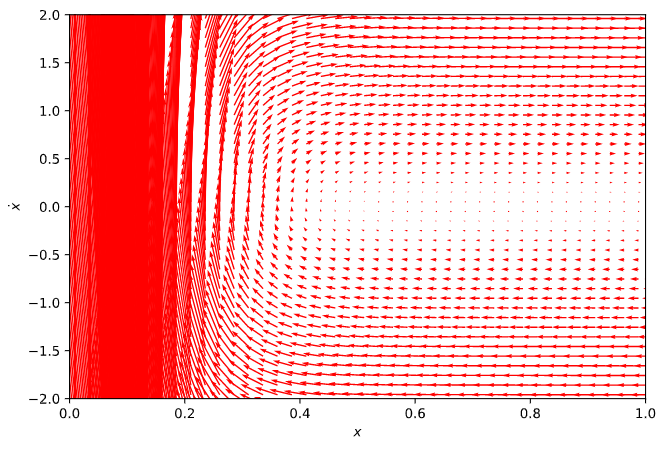
\includegraphics[width=0.55\textwidth]{Images/Chapter5/phase_portrait_obs_naive.png}
\caption{Phase Portrait of naive obstacle avoidance GDS}
\label{fig:chapter5_phase_portrait_obs_naive}
\end{figure}

Here in the figure, state $\yb = [x, \dot{x}]^T$ of this GDS is discretized, and each state corresponds to an arrow that indicates $\yd = [\dot{x}, \ddot{x}]^T$. We shall see that no matter how large the value $\dot{x}$ is, the vertical components of the arrows is the same with a certain value of $x$ , and the collision avoidance only "activates" when the robot is extremely closed to the obstacle and instantly push the robot away from this "barrier". 

\begin{figure}
\centering
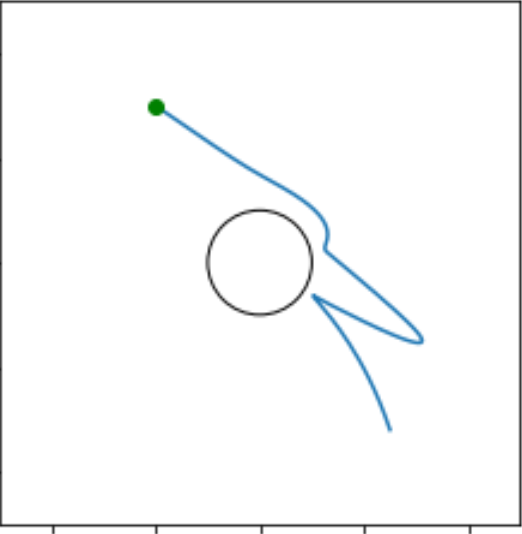
\includegraphics[width=0.55\textwidth]{Images/Chapter5/sim_obs.png}
\caption{Simulation of naive obstacle avoidance behavior}
\label{fig:sim_obs}
\end{figure}

To demonstrate this dynamic behavior, we simulate this collision avoidance and combined it with a target attraction task. The result is shown in 

Indeed, one could choose a mild behavior, for example, let $\Phi(x) = \frac{\alpha}{x}$, however  the stationary point may be unexpected  because this control law always generates a large "force" even if the robot in a relatively safe distance to the obstacle.






%\input{related}
%\input{photoshoot}
%\input{modeling}
%\input{application}
%\input{conclusion}

\appendix

\backmatter

\addcontentsline{toc}{chapter}{\bibname}
\bibliographystyle{abbrv}

% Your bibliography goes here
\bibliography{thesis}

\end{document}
